\chapter*{Introduction}
\label{ch:Introduction}
% This study focuses on capturing emotional dynamics in song lyrics by assigning
% emotion labels to individual stanzas rather than entire songs.
% This approach allows for a more granular analysis of emotional shifts within
% the text.
% The emotion labels correspond to Robert Plutchik's eight primary emotions\textsuperscript{\cite{plutchik1980general}}
% (shown in figure~\ref{fig:primary_emotions}),
% providing a comprehensive range
% for representing various emotional states.\\

\noindent
\begin{minipage}{0.65\textwidth}
    This study focuses on capturing emotional dynamics in song lyrics by assigning
    emotion labels to individual stanzas rather than entire songs.
    This approach allows for a more granular analysis of emotional shifts within
    the text.
    The emotion labels correspond to Robert Plutchik's eight primary emotions\textsuperscript{\cite{plutchik1980general}},
    (figure~\ref{fig:primary_emotions}),
    providing a comprehensive range for representing various emotional states.
\end{minipage}
\hfill
\begin{minipage}{0.27\textwidth}
    \centering
    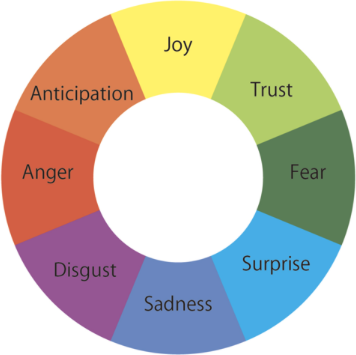
\includegraphics[width=\textwidth]{pictures/plutchik_primary_emotions.png}
    \captionof{figure}{Plutchik's eight primary emotions}
    \label{fig:primary_emotions}
\end{minipage}\\


% \begin{figure}[H]
%     \centering
%     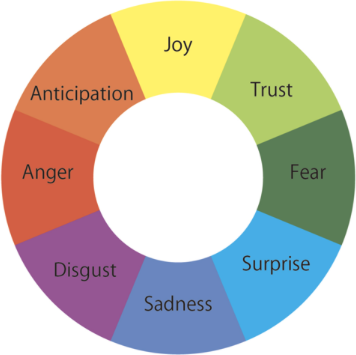
\includegraphics[scale= 0.30]{pictures/plutchik_primary_emotions.png}
%     \caption{Plutchik's eight primary emotions}
%     \label{fig:primary_emotions}
% \end{figure}

The goal of this report is to provide a comprehensive overview of the project,
detailing its methodology, results, and key insights. 
The \textit{Methods} chapter contains a detailed explanation of the data and
procedures used in the project, providing descriptions of each part implemented
in the project.
The \textit{Results} chapter presents an overview of the
obtained outcomes.\\
These results are further explored in the final sections, \textit{Discussion}
and \textit{Conclusions}, which interpret the general findings, present possible
future directions and recap the
primary objectives of the work.